\chapter{Relevant Theory} \label{ch:ns-equations}
\begin{em}
The method shown in the previous section describes a recursive relation that builds the canonical ensemble, which is numerically unstable. In an effort to fix these issues,  a method that utilizes an alternative recursive relation (Eq. (\ref{hatemrr})) will be developed. First, the canonical partition function is rescaled using a set of arbitrary parameters, and the corresponding recursive relation is derived. The set of the parameters is then chosen to enhance the numerical stability of the recursive calculation. To physically motivate a proper choice of the arbitrary parameters, the connection between the canonical partition function and the particle number distribution in the grand canonical ensembles is utilized. Finally, the low-temperature scaling of the error in measuring the temperature of a system with a fixed number of fermions using grand canonical considerations is derived.
\end{em}


\section{Stable Recursion Relation}
The issue with the Borrmann Eq.\@ (\ref{Borrmann}) was the numerical instability. This instability arose from losing the contribution from relevant energy levels along with a sign problem. To fix this, we want to utilize the stable recursion relation Eq.\@ (\ref{hatemrr}) which allows the inclusion of energy levels in the spectrum in any order. To further enhance the numerical stability of this recursion, we introduce the rescaled function $\Tilde{Z}_N$ using a set of arbitrary parameters ${B^N,A_1,...}$ as follows.
\begin{gather}
    \Tilde{Z}_N = B^N Z_N \prod_k A_k \label{ZtildtoZ}\\
    \text{or}\nonumber\\
    Z_N=\frac{\Tilde{Z}_N}{B^N \prod_k A_k}. \label{ZtoZtild}
\end{gather}
By substitution Eq.\@ (\ref{ZtoZtild}) into Eq.\@ (\ref{hatemrr}), we get
\begin{equation}
    Z_N=\frac{\Tilde{Z}_N}{B^N \prod_k A_k} = \frac{\Tilde{Z}_N^{\backslash\{j\}}}{\frac{B^N}{A_j} \prod_k A_k}+e^{-\beta\epsilon_j}\frac{\Tilde{Z}_{N-1}^{\backslash\{j\}}}{\frac{B^{N-1}}{A_j} \prod_k A_k}.
\end{equation}
After some algebra, this becomes
\begin{equation}
   \Tilde{Z}_N=A_j \Tilde{Z}_N^{\backslash\{j\}}+ e^{-\beta\epsilon_j} B \Tilde{Z}_{N-1}^{\backslash\{j\}} A_j.\label{2.6}
\end{equation}
One choice for the coefficients in Eq.\@ (\ref{2.6}) is to choose the parameter $B$ such that $B e^{-\beta\epsilon_F}\approx 1$, where $\epsilon_F$ is the Fermi energy level. The Fermi energy is the level at which all one-particle states with with energy less than the current level are occupied at zero temperature \cite{Kardar}.

For $\epsilon_j\ll\epsilon_F$, we can regulate the effect of the corresponding large factors $B e^{-\beta\epsilon_j}$ by setting $A_j=\frac{e^{\beta\epsilon_j}}{B}$ while for other energy levels we set $A_j=1$. To give these values physical meaning, we can define $B$ and $A_j$ coefficients in terms of the grand canonical occupation probabilities and the corresponding chemical potential. Specifically, we can set $B=e^{\beta\mu}$ and $A=\avg{\bar{n}_j}_{GC}=\frac{1}{1+\exp(-\beta(\epsilon_j-\mu))}$ where $\mu$ is chosen to set the number of particles in the system. At low temperature, $\mu\approx\epsilon_F$. With these definitions, Eq.\@ (\ref{ZtildtoZ}) becomes 
\begin{align}
    \Tilde{Z}_N&=\frac{e^{\beta\mu N} Z_N}{\prod_k \frac{1}{\avg{\bar{n}_k}_{GC}}}\nonumber\\
    &=\frac{e^{\beta\mu N} Z_N}{Z_{GC}}. \label{partnum}
\end{align}
From this equation, we can see that $\Tilde{Z}_N$ is the particle number distribution. This value describes the probability $P_N$ of having $N$ particles in the grand canonical ensemble. Substituting the choices for $B$ and $A_j$ into Eq.\@ (\ref{2.6}) we get
% An important note here is that the division by $A_j$ is to account for the missing energy level $j$. Also, the exponent on the $B$ terms correspond to the number of particles being considered in the original $Z_N^{\backslash\{j\}}$ term. Simplifying this expression gives
% which is the same recursive relation as before, but with the addition of the scaling factors. In order to complete this relationship, an appropriate choice for $A_j$ and $B$ needs to be made. Using Eq.\@ (\ref{PN}) and Eq.\@ (\ref{GCq}), two choices with physical meanings would be $B=e^{\beta\mu}$ and $A=\avg{\bar{n}_j}_{GC}=\frac{1}{1+\exp(-\beta\epsilon_j-\mu)}$. The switch to $j$ for $\avg{\bar{n}_j}$ is only to keep the form of Eq.\@ (\ref{2.6}). The definition is still the same as Eq.\@ (\ref{GCcomplement}). Using these values, Eq.\@ (\ref{2.6}) produces
\begin{align}
    % P_N&=\frac{1}{1+\exp(-\beta(\epsilon_j-\mu))} P_N^{\backslash\{j\}}+ \frac{e^{-\beta\epsilon_j} e^{\beta\mu}}{1+\exp(-\beta(\epsilon_j-\mu))} P_{N-1}^{\backslash\{j\}}\nonumber\\
    % &=\frac{1}{1+\exp(-\beta(\epsilon_j-\mu))} P_N^{\backslash\{j\}}+ \frac{\exp(-\beta(\epsilon_j-\mu))}{1+\exp(-\beta(\epsilon_j-\mu))} P_{N-1}^{\backslash\{j\}}\nonumber\\
    % &=\frac{1}{1+\exp(-\beta(\epsilon_j-\mu))}  P_N^{\backslash\{j\}}+ \frac{1}{1+\exp(\beta(\epsilon_j-\mu))}  P_{N-1}^{\backslash\{j\}}\nonumber\\
    % &=\avg{\bar{n}_j}_{GC}  P_N^{\backslash\{j\}}+ (1-\avg{\bar{n}_j}_{GC}) P_{N-1}^{\backslash\{j\}}\nonumber\\
    P_N&=\avg{\bar{n}_j}_{GC}  P_N^{\backslash\{j\}}+ \avg{n_j}_{GC} P_{N-1}^{\backslash\{j\}} \label{recursiontopb}
\end{align}
where the definition for $\avg{\bar{n}_j}_{GC}$ mentioned above was used and $1-\avg{\bar{n}_j}_{GC}$ is the occupation probability $\avg{n_j}_{GC}=\frac{1}{1+e^{-\beta(\mu-\epsilon_j)}}$.

% Again, $j$ is used to keep the form of Eq.\@ (\ref{recursiontopb}), but is still defined by Eq.\@ (\ref{GCoccprob}). This is a formula to recursively build up $\Tilde{Z}_N$. Next, the definition of $\Tilde{Z}_N$ is found by plugging in the values for $B$ and $A_k$ back into Eq.\@ (\ref{ZtoZtild}) to find
% \begin{align}
%     \Tilde{Z}_N=Z_N B^N \prod_k A_k=Z_N e^{\beta\mu N} \prod_i q_i=\frac{e^{\beta\mu N}Z_N}{Z_{GC}}=P(N).
% \end{align}
% This shows that with the right choice of $A_j$ and $B$, the recursion relationship for $\Tilde{Z}_N$ gives the particle number distribution needed in Eq.\@ (\ref{partnumdist}). The recursive relationship can now be written as
% \begin{gather}
%     \Tilde{Z}_N=\avg{q_j}_{GC} \Tilde{Z}_N^{\backslash\{j\}}+ \avg{n_j}_{GC} \label{Ztildetopb} \Tilde{Z}_{N-1}^{\backslash\{j\}}\\
%     P_N=\avg{q_j}_{GC} P_N^{\backslash\{j\}}+ \avg{n_j}_{GC} P_{N-1}^{\backslash\{j\}} \label{pbback}
% \end{gather}
Eq.\@ (\ref{recursiontopb}) could be viewed as the Poisson binomial recursive relation
\begin{equation}
    P_N=q_j  P_N^{\backslash\{j\}}+ p_j P_{N-1}^{\backslash\{j\}} \label{pbrr}
 \end{equation}
for a set of individual success probabilities $\{p_j\}$ and their complements $\{q_j\}$. Here, the $p_j\equiv \avg{n_j}_{GC}$ terms represent the success probability of occupying energy level $j$ in the grand canonical ensemble. Likewise, $q_j\equiv \avg{\bar{n}_j}_{GC}$. The Poisson binomial distribution is a generalized form of the binomial distribution. The binomial distribution contains $M$ trials with a fixed success probability $p$ for each trial. The Poisson binomial distribution, on the other hand, allows for the probability $p$ to change with each trial. In the language of the coin toss example, the binomial distribution would be the result of using the same coin for $M$ trials while the Poisson binomial distribution would be the result of changing the coin each trial. In the binomial distribution, the average value of successes (say, heads), would be the sum of all $p$ values, or $p$ time $M$ since the probability stays constant. In the Poisson binomial distribution, this average would come from summing all of the values for $p_j$ since they are allowed to vary. 

This recursion has many interesting properties. To start, it adds on a value to the distribution each iteration. When at position $N+1$, the $p_j P_{N-1}^{\backslash\{j\}}$ term still contributes a nonzero value to the probability. This means that iterating over all possible $j$ values for $p_j$ and $q_j$ will give a distribution that is $j+1$ values long. This can be viewed as the general form of a Pascal triangle since Pascal's triangle applies to the binomial distribution. 

Let $P_j(N)$ be the probability of having $N$ successes given $j$ individual events. 
\begin{equation*}
    P_j(N)=q_j P_{j-1}(N)+ p_j P_{j-1}(N-1). \label{pbrrshort}
\end{equation*} 
To build some intuition of this, let us consider another short example. To start, let the probability distribution be
\begin{gather}
    p_j\in \left\{1,\frac{1}{2},\frac{1}{3},\frac{1}{6}\right\}\nonumber
\end{gather}
and thus, its complement is
\begin{gather}
    q_j \in \left\{0,\frac{1}{2},\frac{2}{3},\frac{5}{6}\right\}\nonumber
\end{gather}
where each term in the set corresponds to the probability that a particle occupies (or doesn't occupy) that state. By summing the values in the probability distribution, the average number of successes is $\sum_j p_j=\avg{N}=2$. From here, the recursive relationship can be initialized with the value of $P_0(0)=1$. The calculation can then continue until all values in the probability set are used. This is done to show
\begin{gather*}
    P_1(0)=q_1P_{0}(0)=(0)(1)=0\\
    P_1(1)=p_1 P_{0}(0)=(1)(1)=1.
\end{gather*}
So this first step of the recursion gives
\begin{equation*}
    P_1(0)=0, P_1(1)=1.
\end{equation*}
Continuing onto the next step,
\begin{gather*}
    P_1(0)=q_2 P_{1}(0)= \qty(\frac{1}{2})(0)=0\\
    P_2(1)=p_2 P_{1}(0)+q_2 P_{1}(1)=\qty(\frac{1}{2})(0)+\qty(\frac{1}{2})(1)=\frac{1}{2}\\
    P_2(2)=p_2 P_{1}(1)=\qty(\frac{1}{2})(1)=\frac{1}{2}
\end{gather*}
gives
\begin{gather*}
    P_2(0)=0, P_2(1)=\frac{1}{2}, P_2(2)=\frac{1}{2}.
\end{gather*}
The next step gives
\begin{gather*}
    P_3(0)=q_3 P_2(0)=\qty(\frac{2}{3})(0)=0\\
    P_3(1)=p_3 P_{2}(0)+q_3 P_{2}(1)=\qty(\frac{1}{3})(0)+\qty(\frac{2}{3})\qty(\frac{1}{2})=\frac{1}{3}\\
    P_3(2)=p_3 P_{2}(1)+q_3 P_{2}(2)=\qty(\frac{1}{3})\qty(\frac{1}{2})+\qty(\frac{2}{3})\qty(\frac{1}{2})=\frac{1}{2}\\
    P_3(3)=p_3 P_{2}(2)=\qty(\frac{1}{3})\qty(\frac{1}{2})=\frac{1}{6}\\
\end{gather*}
This yields,
\begin{equation*}
    P_3(0)=0, P_3(1)=\frac{1}{3}, P_3(2)=\frac{1}{2}, P_3(3)=\frac{1}{6}
\end{equation*}
Continuing,
\begin{gather*}
    P_4(0)=q_4 P_3(0)=\qty(\frac{5}{6})(0)=0\\
    P_4(1)=p_4 P_{3}(0)+q_4 P_{3}(1)=\qty(\frac{1}{6})(0)+\qty(\frac{5}{6})\qty(\frac{1}{3})=\frac{10}{36}\\
    P_4(2)=p_4 P_{3}(1)+q_4 P_{3}(2)=\qty(\frac{1}{6})\qty(\frac{1}{3})+\qty(\frac{5}{6})\qty(\frac{1}{2})=\frac{17}{36}\\
    P_4(3)=p_4 P_{3}(2)+q_4 P_{3}(3)=\qty(\frac{1}{6})\qty(\frac{1}{2})+\qty(\frac{5}{6})\qty(\frac{1}{6})=\frac{8}{36}\\
    P_4(4)=p_4 P_{3}(3)=\qty(\frac{1}{6})\qty(\frac{1}{6})=\frac{1}{36}
\end{gather*}
Since there are no more probabilities to include, the final distribution has been found to be
\begin{equation*}
    P_4(0)=0, P_4(1)=\frac{10}{36}, P_4(2)=\frac{17}{36}, P_4(3)=\frac{8}{36}, P_4(4)=\frac{1}{36}.
\end{equation*}
This solution can be visualized as a triangle as seen in Fig.\@ (\ref{fig:Poisson Binomial Triangle}). 
\begin{figure}[H]
    \centering
    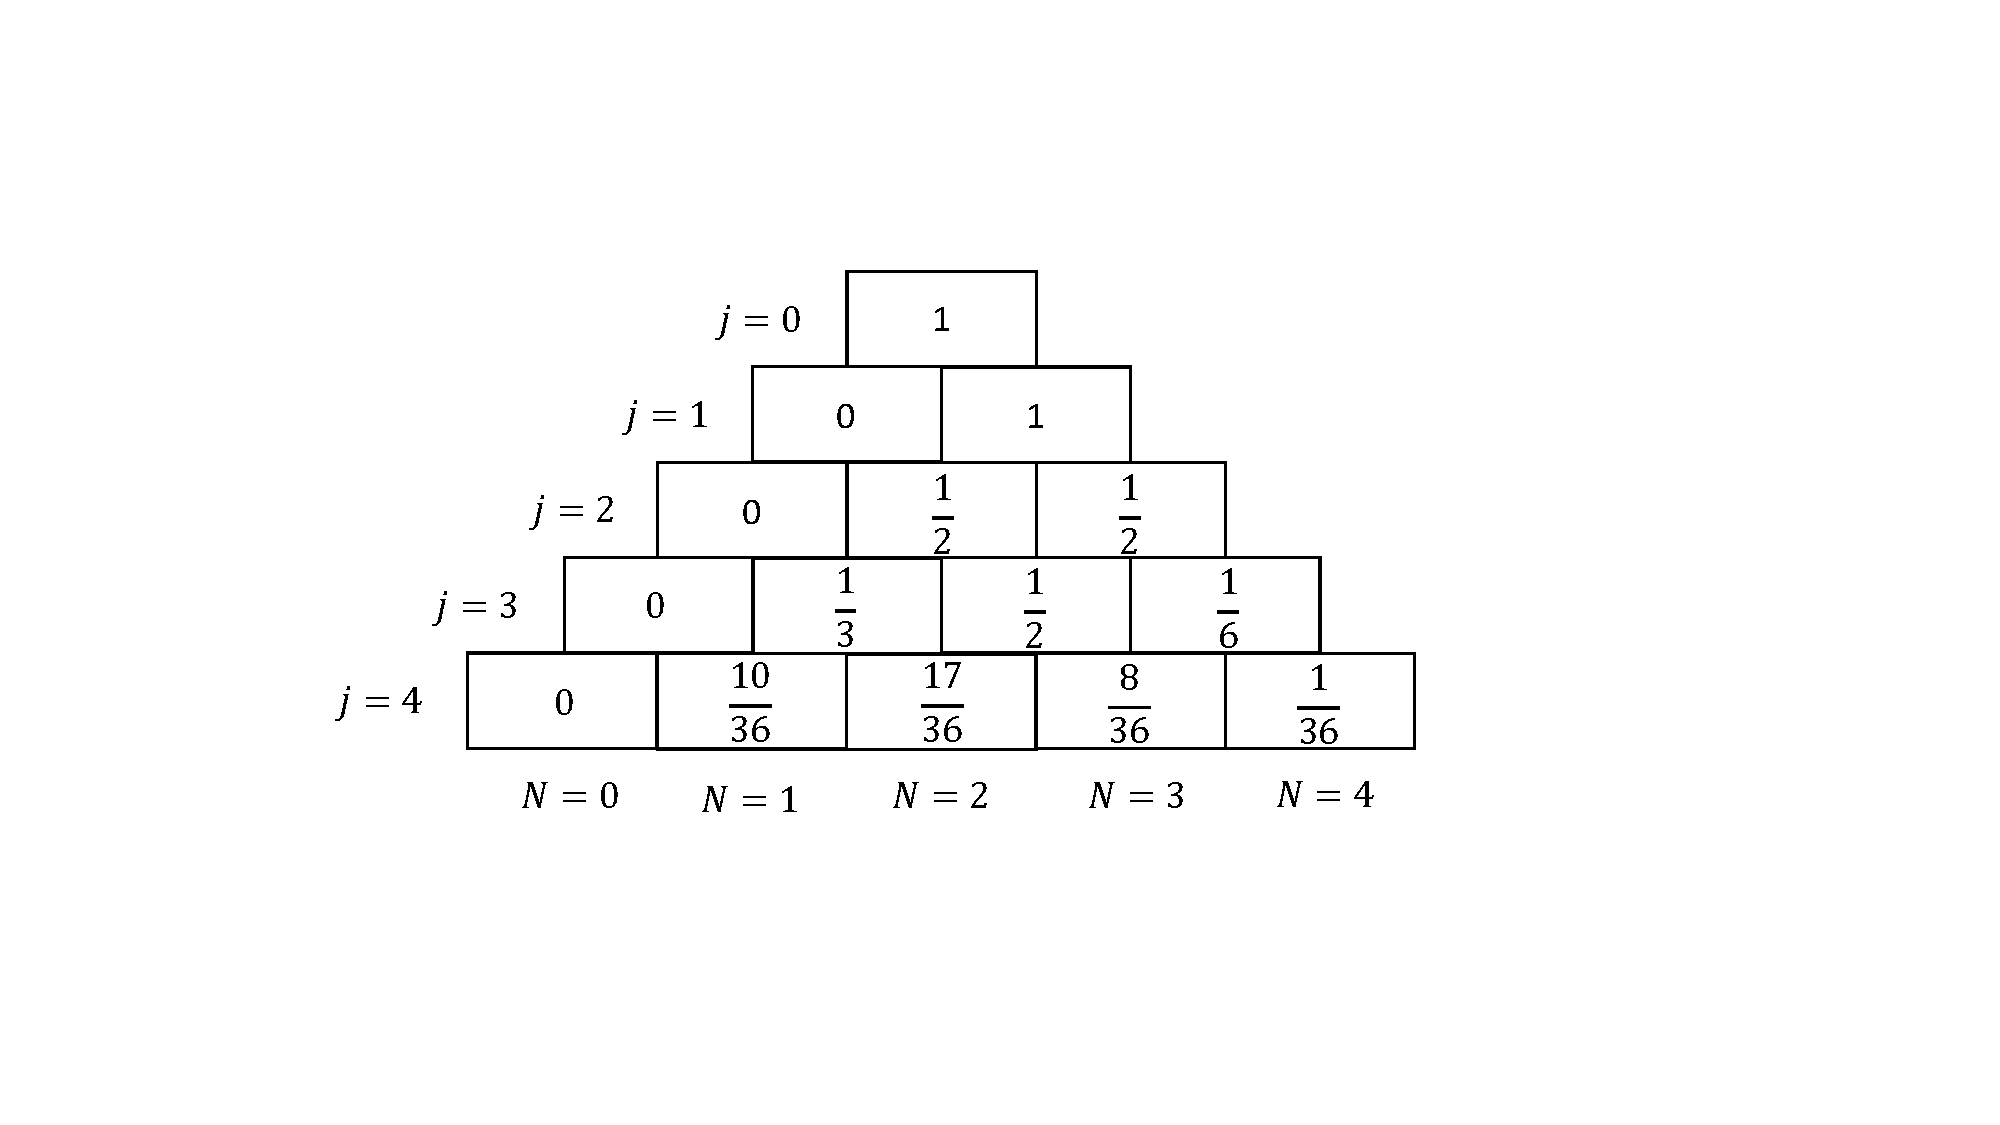
\includegraphics[scale=0.55]{figures/pdf/PBTriangle.pdf}
    \caption{The Poisson binomial triangle for the example considered above. After using the recurrence relation to include all probability levels, the base of the triangle gives the particle number distribution for the system.}
    \label{fig:Poisson Binomial Triangle}
\end{figure}
The generalized pascal triangle is shown in Fig.\@ (\ref{fig:General Poisson Binomial Recursion}).
\begin{figure}[H]
    \centering
    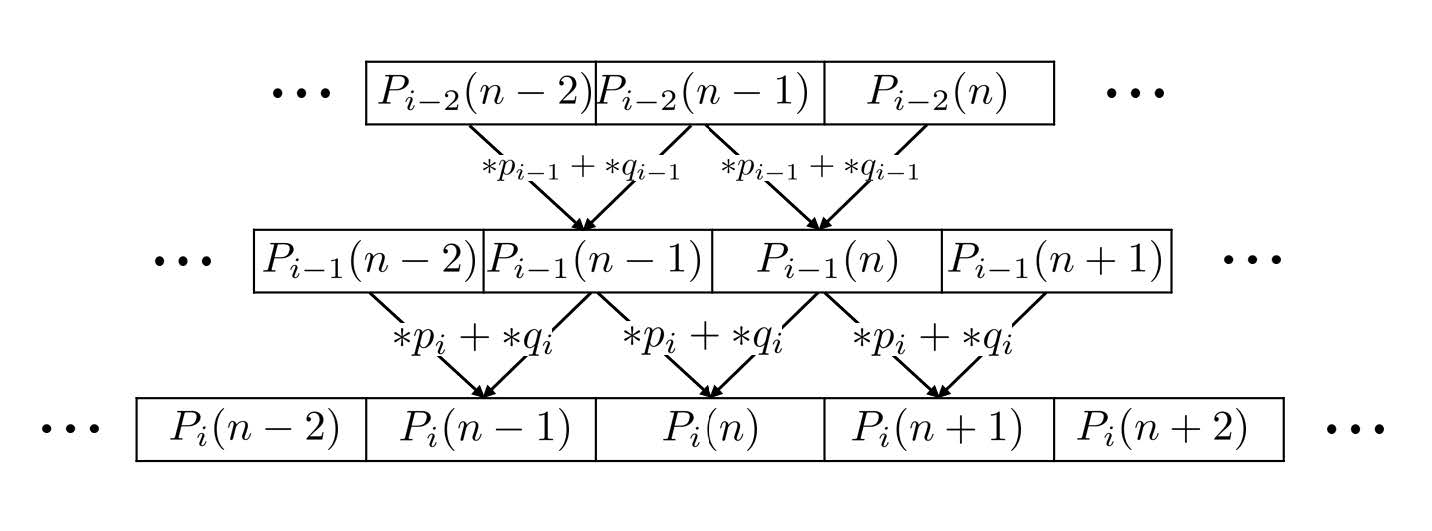
\includegraphics[scale=0.8]{figures/pdf/PBrecursion.jpg}
    \caption{The generalized Pascal triangle. Here, $i=j$ denotes the number of probabilites included from the distribution, $p$ denotes the probabilities, and $q$ denotes the complimentary probability. $P_i(n)$ is term $n$ in the probability distribution that contains $i$ of the probabilities. Each new term is the sum of the arrows pointing to it. Each arrow is multiplied ($*$) by $p_i$ or $q_i$.}
    \label{fig:General Poisson Binomial Recursion}
\end{figure}
In this case, $\avg{N}=\sum_N N P(N)=2$ where $P(N)=P_4(N)$ for this example. Moreover, the variance $\sigma^2=\sum_N P(N)\qty[\avg{N^2}-\avg{N}^2]=\frac{11}{18}$ can also be calculated as $\sigma^2=\sum_j p_j q_j=\frac{11}{18}$. After obtaining $P(N)$, one can get the corresponding $Z_N$ according to Eq.\@ (\ref{partnum}) by writing 
\begin{equation}
    Z_N=P(N) Z_{GC} e^{-\beta\mu N}. \label{ZCasZGC}
\end{equation}
One advantage of applying the recursion relation on $P(N)$ instead of $Z_N$, like in Eq.\@ (\ref{hatemrr}), is that $P(N)$ is bounded between $0$ and $1$ while $Z_N$ is not. With the proper choice of $\mu$, the desired $P(N)$ value is expected to be around the peak of the particle number distribution, thus suffers less from the precision limitation that showed up in Eq.\@ (\ref{Borrmann}). 



\section{Occupation Probability from recursion}
The occupation probability in the canonical ensemble can be found from applying Eq.\@ (\ref{partnum}) and $\Tilde{Z}_N=P_N$ to Eq.\@ (\ref{hatemrr}). The canonical occupation probability is found from Eq.\@ (\ref{hatemrr}) by dividing by the full partition function such that 
\begin{align}
    1=\frac{Z_N^{\backslash\{j\}}}{Z_N}+e^{-\beta\epsilon_j}\frac{Z_{N-1}^{\backslash\{j\}}}{Z_N}.
\end{align}
The second term on the right hand side is the canonical occupation probability $\avg{n_j}_C$ \cite{Hatem2020}. Using the relationships derived in the previous section, we can write
\begin{align}
    \avg{n_j}_C&=e^{-\beta\epsilon_j}\frac{Z_{N-1}^{\backslash\{j\}}}{Z_N}\nonumber\\
    &=\frac{e^{-\beta\epsilon_j}P_N^{\backslash\{j\}}e^{-\beta\mu(N-1)}Z_{GC}^{\backslash\{j\}}}{e^{-\beta\mu N} P_N Z_{GC}}\nonumber\\
    &=\frac{e^{-\beta(\epsilon_j-\mu)} P_N^{\backslash\{j\}}}{Z_{GC}(\{j\}) P_N}\nonumber\\
    &=\frac{e^{-\beta(\epsilon_j-\mu)}}{1+e^{-\beta(\epsilon_j-\mu)}} \frac{P_N^{\backslash\{j\}}}{P_N}\nonumber\\
    &=\avg{n_j}_{GC} \frac{P_N^{\backslash\{j\}}}{P_N}. \label{rroccprob}
\end{align}
The term $Z_{GC}(\{j\})$ is the grand canonical ensemble for only level $j$ and the definition of the grand canonical occupation probability used from Eq.\@ (\ref{GCoccprobab}). Eq.\@ (\ref{rroccprob}) shows that the canonical occupation probabilities can be found from the grand canonical occupation probabilities and particle number distribution. 


\section{Temperature Extraction}
\label{section:TemperatureExtraction}
With the occupation probabilities, the temperature can be extracted by fitting the probabilities to a distribution. Since we are interested in the error made from fitting a canonical distribution to a grand canonical distribution, the grand canonical occupation probability given by Eq.\@ (\ref{GCoccprobab}) is used. The chemical potential is fixed in this equation by using the average number of particles. This allows for the extraction of the grand canonical temperature $\beta^*$. This process is done by minimizing a $\chi^2$ least-squares difference function defined as 
\begin{equation}
    \chi^2=\sum_j(\avg{n_j}_{GC}-\avg{n_j}_C)^2. \label{chisq}
\end{equation}
With $\mu$ fixed, the only variable in this equation is $\beta^*$. Since the equation is dependent only on $\beta^*$, the first and second derivatives can be calculated and used to find the minimum. The full calculation is performed in Appendix B. Let $p_j=\avg{n_j}_{GC}$, $q_j=\avg{\bar{n}_j}_{GC}$, and $n_j=\avg{n_j}_C$ to simplify the calculations. The important results are 
\begin{gather}
    \frac{d\chi^2}{d\beta^*}=\sum_j -2(p_j-n_j)p_j q_j \epsilon_j+\sum_j 2(p_j-n_j)p_j q_j C_1\\
    \frac{d^2\chi^2}{d\beta^{*2}}=2\sum_j\Biggr[(\epsilon_j-C_1)^2[(p_j-n_j)p_jq_j(q_j-p_j)+p_j^2q_j^2]\nonumber\\
    \ \ \ \ \ \ +(p_j-n_j)p_jq_j(C_1C_3+C_2)\Biggr]\\
    C_1=\frac{\sum_j \epsilon_j p_j q_j}{\sum_j p_j q_j}\\
    C_2=\frac{\sum_j \epsilon_j p_j q_j(p_j - q_j)(\epsilon_j-C_1)}{\sum_j p_j q_j}\\
    C_3=\frac{\sum_j p_j q_j(q_j-p_j)(\epsilon_j-C_1)}{\sum_j p_j q_j}.
\end{gather}
With both derivatives available, Newton's method of optimization is used to find the correct value of $\beta^*$. This method involves using 
\begin{equation}
    \beta_{\text{update}}^*=\beta_{\text{previous}}^*-\qty(\frac{d}{d\beta^*}\chi^2)\qty({\frac{d^2}{d\beta^{*2}}\chi^2})^{-1}
\end{equation}
to iterate until the minimum is found to a desired level or numerical precision.

\section{Degenerate energy spectra}
The Poisson binomial recursive method was developed on the assuming a nondegenerate energy spectrum. This assumption is not the case in the cold atom experiments mentioned in Chapter 1. In two or three dimensional harmonic or quadratic traps, there will be some number of degeneracy for each level and the spectrum does not necessarily have the same spacing as their one dimensional counterparts. For this reason it is necessary that degeneracy be considered. 


\subsection{Filled Degenerate Fermi Level}
The first case to consider is when the Fermi level is degenerate and filled for large $\beta$. In this case, for sufficiently large $\beta$, the thermodynamical properties of the  system are governed by the excitation from the Fermi level to the first excited level. Since all other levels are filled or empty, let us relabel our energy levels such that $i=0$ denotes the Fermi level and $i=1$ denotes the first excited state. Let the degeneracy of level $i$ be $g_i$. In a system of $N$ particles with a filled Fermi level, there are $g_0$ particles between the levels $\epsilon_0$ and $\epsilon_1$, where $\epsilon_0$ is the energy of the Fermi level and $\epsilon_1$ is the energy of the first excited state. The canonical partition function of $k$ particles for a single level of energy $\epsilon_i$ and degeneracy $g_i$ where $k\leq g_i$ is 
\begin{equation}
    Z_k(\epsilon_i;g_i)={g_i \choose k} e^{-k\beta\epsilon_i}.
    \label{eq:ZNsinglelevel}
\end{equation}
The Boltzmann factor $e^{-k\beta\epsilon_i}$ is the same across all ${g_i \choose k}$ possible occupations. Since there are only two levels of interest in this case, the simple example in Section 1.3 can be revisited. Consider that there is one particle in a system where the Fermi level has degeneracy $g_0$ and energy $\epsilon_0$ and the first excited state has degeneracy $g_1$ and energy $\epsilon_1$. For convenience, the energy spectrum can be redefined as
\begin{equation}
    \epsilon_0 \xrightarrow[]{} 0\ \ \ \ \ \epsilon_1\xrightarrow[]{}\Delta_0=\epsilon_1-\epsilon_1.\nonumber
\end{equation}
The partition function for this case can be written from Eqs. (\ref{eq:ZNsinglelevel}) and (\ref{eq:ZNcombine}) to yield
\begin{align}
    Z_{g_0}(0,\Delta_0;g_0,g_1)&=\sum_{k=0}^{\text{min}(g_1,g_0)} Z_k(\Delta_0,g_1)Z_{g_0-k}(0,g_0)\nonumber\\
    &=\sum_{k=0}^{\text{min}(g_1,g_0)} {g_1 \choose k}{g_0\choose g_0-k} e^{-\beta \epsilon_0 k}e^{-\beta \epsilon_1 k}\nonumber\\
    &=\sum_{k=0}^{\text{min}(g_1,g_0)} {g_1 \choose k}{g_0\choose g_0-k} e^{-\beta \Delta_0 k}
\end{align}
where the $\text{min}(g_1,g_0)$ represents the minimum of the two values. The minimum is used here because there can only be as many particles as there are available positions in the energy level. For non degenerate case, this would be one, but for the degenerate case, this can be any positive integer value up to the level degeneracy. The canonical occupation probability can be calculated the same as before by leaving out an energy level and multiplying by its Boltzmann factor. This results in 
\begin{align}
    \avg{n_0}_{g_0}&=\frac{e^{-\beta \epsilon_0}Z_{g_0-1}(0,\Delta_0;g_0-1,g_1)}{Z_{g_0}(0,\Delta_0;g_0,g_1)}\nonumber\\
    &=\frac{\sum_{k=0}^{\text{min}(g_1,g_0-1)} {g_1 \choose k}{g_0\choose g_0-1-k} e^{-\beta \Delta_0 k}}{\sum_{k=0}^{\text{min}(g_1,g_0)} {g_1 \choose k}{g_0\choose g_0-k} e^{-\beta \Delta_0 k }}\nonumber\\
    &=\frac{{g_1\choose 0}{g_0-1\choose g_0-1}+{g_1 \choose 1}{g_0-1\choose g_0-2}e^{-\beta\Delta_0}+{g_1\choose 2}{g_0-1\choose g_0-3}e^{-2\beta\Delta_0}+...}{{g_1\choose 0}{g_0\choose g_0}+{g_1 \choose 1}{g_0\choose g_0-1}e^{-\beta\Delta_0}+{g_1\choose 2}{g_0-1\choose g_0-2}e^{-2\beta\Delta_0}+...}\nonumber\\
    &=\frac{1+g_1(g_0-1)e^{-\beta\Delta_0}+\frac{g_1(g_1-1)(g_0-1)(g_0-2)}{4}e^{-2\beta\Delta_0}+...}{1+g_0g_1e^{-\beta\Delta_0}+\frac{g_1(g_1-1)g_0(g_0-1)}{4}e^{-2\beta\Delta_0}+...}.
\end{align}
Similarly, for the first excited state,
\begin{align}
    \avg{n_1}_{g_0}&=\frac{e^{-k\epsilon_1} Z_{g_0-1}(0,\Delta_0;g_0,g_1-1)}{Z_{g_0}(0,\Delta_0;g_0,g_1)}\nonumber\\
    &=\frac{e^{-k\Delta_0}\sum_{k=0}^{\text{min}(g_1-1,g_0-1)} {g_1-1\choose k}{g_0 \choose k+1} e^{-k\beta\Delta_0}}{\sum_{k=0}^{\text{min}(g_1,g_0)} {g_1\choose k}{g_0 \choose k} e^{-k\beta\Delta_0}}\nonumber\\
    &=\frac{{g_1-1\choose 0}{g_0\choose 1} e^{-\beta\Delta_0} +{g_1-1\choose 1}{g_0\choose 2} e^{-2\beta\Delta_0}+{g_1-1\choose 2}{g_0\choose 3}e^{-3\beta\Delta_0}+...}{{g_0\choose 0}{g_1\choose 0}+{g_0\choose 1}{g_1\choose 1}e^{-\beta\Delta_0}+{g_0\choose 2}{g_1\choose 2}e^{-2\beta\Delta_0}+...}\nonumber\\
    &=\frac{g_0e^{-\beta\Delta_0}+\frac{(g_1-1)g_0(g_0-1)}{2}e^{-2\beta\Delta_0}+...}{1+g_0g_1 e^{-\beta\Delta_0}+\frac{g_1(g_1-1)g_0(g_0-1)}{4}e^{-2\beta\Delta_0}+...}.
\end{align} 
Like before, the chemical potential can be found by using the grand canonical probabilities $p_0$ and $p_1$ such that,
\begin{gather}
    p_0=\frac{1}{1+e^{\beta^*(\epsilon_0-\mu)}}=\frac{1}{1+e^{-\beta^* \mu}} \label{grcn}\\
    p_1=\frac{1}{1+e^{\beta^*(\epsilon_0-\mu)}}=\frac{1}{1+e^{\beta^*(\Delta_0-\mu)}}\\
    p_0g_0+p_1g_1=g_0.
\end{gather}
Plugging everything in gives
\begin{gather}
    g_0=\frac{g_0}{1+e^{\beta^*(\epsilon_0-\mu)}}=\frac{1}{1+e^{-\beta^*\mu}}+\frac{g_1}{1+e^{\beta^*(\epsilon_0-\mu)}}=\frac{1}{1+e^{\beta^*(\Delta_0-\mu)}}\nonumber\\
    1+e^{\beta^*\Delta_0} e^{-\beta^*\mu}+\frac{g_1}{g_0}(1+e^{-\beta^*\mu})=(1+e^{-\beta^*\mu})(1+e^{\beta^*\Delta_0} e^{-\beta^* \mu})\nonumber\\
    1+e^{-\beta^*\mu}(\frac{g_1}{g_0}+e^{\beta^*\Delta_0})+\frac{g_1}{g_0}=1+e^{-\beta^*\mu}+e^{\beta^*\Delta_0}e^{-\beta^*\mu}+e^{-2\beta^*\mu}e^{\beta^*\Delta_0}\nonumber\\
    0=(e^{-\beta^*\mu})^2 e^{\beta^*\Delta_0} +e ^{-\beta^*\mu}(1-\frac{g_1}{g_0})-\frac{g_1}{g_0}.
\end{gather}
This is a simple quadratic equation so there will be two solutions. To have a real solution, the positive root is kept resulting in
\begin{align}
    e^{-\beta^*\mu}&=\frac{(\frac{g_1}{g_0}-1)\pm\sqrt{(\frac{g_1}{g_0}-1)^2+4e^{\beta^*\Delta_0}\frac{g_1}{g_0}}}{2e^{\beta^*\Delta_0}}\nonumber\\
    &=\frac{e^{-\beta^*\Delta_0}}{2}(\frac{g_1}{g_0}-1)\pm \frac{1}{2}\sqrt{e^{-2\beta^*\Delta_0} (\frac{g_1}{g_0}-1)^2+ 4e^{-\beta^*\Delta_0}\frac{g_1}{g_0}}.
\end{align}
Just like the simple example we saw in Chapter 1, we set the canonical and grand canonical probabilities to be equal, such that $\avg{n_0}_{g_0}=p_0$. This gives 
\begin{align}
    \frac{1}{\avg{n_0}_{g_0}}-1=\frac{1}{p_0}-1=1+e^{-\beta^*\mu}-1=e^{-\beta^*\mu} .
\end{align}
Now there is a connection to the grand canonical probability to the canonical probability for the degenerate case. Setting the two $e^{-\beta^*\mu}$ terms equal to one another yields
\begin{gather}
    \frac{1}{\avg{n_0}_{g_0}}-1=\frac{e^{-\beta^*\Delta_0}}{2}(\frac{g_1}{g_0}-1)\pm \frac{1}{2}\sqrt{e^{-2\beta^*\Delta_0} (\frac{g_1}{g_0}-1)^2+ 4e^{-\beta^*\Delta_0}\frac{g_1}{g_0}}\nonumber\\
    2\frac{1-\avg{n_0}_{g_0}}{\avg{n_0}_{g_0}}-e^{-\beta^*\Delta_0}(\frac{g_1}{g_0}-1)=\sqrt{e^{-2\beta^*\Delta_0} (\frac{g_1}{g_0}-1)^2+ 4e^{-\beta^*\Delta_0}\frac{g_1}{g_0}}\nonumber\\
    4\qty(\frac{1-\avg{n_0}_{g_0}}{\avg{n_0}_{g_0}})^2-4e^{-\beta^*\Delta_0}\qty(\frac{g_1}{g_0}-1) \frac{1-\avg{n_0}_{g_0}}{\avg{n_0}_{g_0}}+e^{-2\beta^*\Delta_0} \qty(\frac{g_1}{g_0}-1)^2\nonumber\\ 
    \ \ \ \ \ \ \  =e^{-2\beta^*\Delta_0} (\frac{g_1}{g_0}-1)^2+ 4e^{-\beta^*\Delta_0}\frac{g_1}{g_0} \nonumber\nonumber\\
    0=4\qty(\frac{1-\avg{n_0}_{g_0}}{\avg{n_0}_{g_0}})^2- 4e^{-\beta^*\Delta_0}\qty(\qty(\frac{g_1}{g_0}-1)\frac{1-\avg{n_0}_{g_0}}{\avg{n_0}_{g_0}}+\frac{g_1}{g_0})\nonumber\\
    4\qty(\frac{1-\avg{n_0}_{g_0}}{\avg{n_0}_{g_0}})^2=4e^{-\beta^*\Delta_0}\qty(\qty(\frac{g_1}{g_0}-1)\frac{1-\avg{n_0}_{g_0}}{\avg{n_0}_{g_0}}+\frac{g_1}{g_0})\nonumber\\
    e^{\beta^* \Delta_0}=\frac{1-\avg{n_0}_{g_0}}{\avg{n_0}_{g_0}}(\frac{g_1}{g_0}-1)+\qty(\frac{1-\avg{n_0}_{g_0}}{\avg{n_0}_{g_0}})^2\frac{g_1}{g_0}.
\end{gather}
With this definition, $\frac{1-\avg{n_0}_{g_0}}{\avg{n_0}_{g_0}}$ terms are worked out and plugged in. This is done in Appendix C.1. An important note for these calculations is that terms greater than $\mathcal{O}\qty(e^{-2\beta \Delta_0})$ are neglected because they will be sufficiently small at low temperature. Using Eqs.\@ (\ref{C8}) and (\ref{C9}),
\begin{align}
    e^{\beta^* \Delta_0}&=\frac{e^{\beta\Delta_0}}{g_1}\qty(1+\frac{(g_1+1)(g_0-1)}{2}e^{-\beta\Delta_0})\qty(\frac{g_1}{g_0}-1)\nonumber\\
    &\ \ \ \ \ \ \ \ \ \ +\frac{e^{2\beta\Delta_0}}{g_1^2}\qty(1+(g_1+1)(g_0-1)e^{-\beta\Delta_0})\frac{g_1}{g_0}\nonumber\\
    &=\frac{e^{2\beta\Delta_0}}{g_1g_0}\qty((g_1-g_0)e^{-\beta\Delta_0}+1+(g_1+1)(g_0-1)e^{-\beta\Delta_0})\nonumber\\
    &=\frac{e^{2\beta\Delta_0}}{g_1g_0}\qty((g_1g_0-1)e^{-\beta\Delta_0}+1)\\
    \beta^*\Delta_0&=2\beta\Delta_0-\ln(g_0g_1)+\ln\qty((g_1g_0-1)e^{-\beta\Delta_0}+1).
\end{align}
Since $e^{-\beta\Delta_0}$ is small, the third term on the right hand size can be approximated using $\ln(1+x)\approx x$, for $x\ll1$. This yields
\begin{align}
    \beta^*\Delta_0&=2\beta\Delta_0-\ln\qty(g_0g_1)+(g_1g_0-1)e^{-\beta\Delta_0}\nonumber\\
    \beta^*&=2\beta-\frac{\ln\qty(g_0g_1)}{\Delta_0}+\frac{g_1g_0-1}{\Delta_0}e^{-\beta\Delta_0}.
\end{align} 
This is the relationship between the canonical temperature and the grand canonical temperature. This can be rewritten in terms of the error of the grand canonical $\beta^*$ value. For this, consider 
\begin{align}
    \frac{\beta^*-\beta}{\beta}=\frac{\delta\beta}{\beta}=1-\frac{\ln(g_0g_1)}{\beta\Delta_0}+\frac{(g_1g_0 - 1)}{\beta \Delta_0}e^{-\beta\Delta_0}. \label{filldegen}
\end{align}
This equation should give the same results when the degeneracies are removed. Doing this gives
\begin{gather}
    g_0=g_1=1\nonumber\\
    \frac{\delta\beta}{\beta}=1-\frac{\ln(1)}{C_1}+\frac{(1)(1)-1}{C_2}=1. \label{filldegencheck}
\end{gather}
This is the condition for the nondegenerate case, so the filled degenerate fermi level case is consistent with the nondegenerate case. 
\subsection{Partially Filled Degenerate Fermi Level}
Turning to the case of a partially filled degenerate energy spectrum, consider that the Fermi level is partially filled. This setup requires considering both the level above and below the Fermi level. The energy spectrum can be rewritten as 
\begin{gather}
    \epsilon_0 \xrightarrow[]{} 0\nonumber\\
    \epsilon_1 \xrightarrow[]{} \Delta_0=\epsilon_1-\epsilon_0\nonumber\\
    \epsilon_{-1} \xrightarrow[]{} -\Delta_{-1}=\epsilon_{-1}-\epsilon_0.\nonumber
\end{gather}
The number of particles in the partially filled level will be denoted as $\ell$. The partition function for this case is 
\begin{align}
    &Z_{g_{-1}+\ell}(-\Delta_{-1},0,\Delta;g_{-1},g_0,g_1) = e^{g_{-1}\beta\Delta_{-1}} \Biggr[{g_0\choose \ell}+g_1{g_0\choose \ell-1}e^{-\beta\Delta_0} \nonumber\\
    &\quad +g_{-1}{g_0\choose \ell+1}e^{-\beta\Delta_{-1}} +\frac{g_1(g_1-1)}{2} {g_0\choose \ell-2}e^{-2\beta\Delta_0}\nonumber\\ 
    &\quad +\frac{g_{-1}(g_{-1}-1)}{2} {g_0\choose \ell+2} e^{-2\beta\Delta_{-1}} +g_1g_{-1}{g_0\choose \ell} e^{-\beta(\Delta_0+\Delta_{-1})} \Biggr]\nonumber\\
    &\ \ =e^{g_{-1}\beta\Delta_{-1}} {g_0\choose \ell} \Biggr[1+ \frac{g_1 \ell}{g_0-\ell+1} e^{-\beta\Delta_0} +\frac{g_{-1}(g_0-\ell)}{\ell+1} e^{-\beta\Delta_{-1}} \nonumber\\
    &\quad+\frac{g_1(g_1-1)}{2} \frac{\ell(\ell-1)}{(g_0+\ell+1)(g_0+\ell+2)}e^{-2\beta\Delta_0} \nonumber\\
    &\quad+\frac{g_{-1}(g_{-1}-1)}{2} \frac{(g_0-\ell)(g_0-\ell-1)}{(\ell+1)(\ell+2)} e^{-2\beta\Delta_{-1}}+g_1g_{-1}e^{-\beta(\Delta_0+\Delta_{-1})}\Biggr].
\end{align}
As before, the partition function can be found for states with one particle removed. For level $i=-1$,
\begin{align}
    &Z_{g_{-1}+\ell-1}(-\Delta_{-1},0,\Delta_0;g_{-1}-1,g_0,g_1)=e^{(g_{-1}-1)\beta\Delta_{-1}} {g_0\choose \ell} \Biggr[1+\frac{g_1 \ell}{g_0-\ell+1} e^{-\beta\Delta_0} \nonumber\\
    &\quad +\frac{(g_{-1}-1)(g_0-\ell)}{\ell+1} e^{-\beta\Delta_{-1}}+\frac{g_1(g_1-1)}{2} \frac{\ell(\ell-1)}{(g_0+\ell+1)(g_0+\ell+2)}e^{-2\beta\Delta_0} \nonumber\\
    &\quad+\frac{(g_{-1}-1)(g_{-1}-2)}{2} \frac{(g_0-\ell)(g_0-\ell-1)}{(\ell+1)(\ell+2)} e^{-2\beta\Delta_{-1}}+g_1(g_{-1}-1)e^{-\beta(\Delta_0+\Delta_{-1})}\Biggr].
\end{align}
For level $i=0$,
\begin{align}
    &Z_{g_{-1}+\ell-1}(-\Delta_{-1},0,\Delta_0;g_{-1},g_0-1,g_1)=e^{g_{-1}\beta\Delta_{-1}} {g_0-1\choose \ell-1} \Biggr[1+\frac{g_1 (\ell-1)}{g_0-\ell-1} e^{-\beta\Delta_0}\nonumber\\
    &\quad+\frac{g_{-1}(g_0-\ell)}{\ell} e^{-\beta\Delta_{-1}} +\frac{g_1(g_1-1)}{2} \frac{(\ell-1)(\ell-2)}{(g_0+\ell+1)(g_0+\ell+2)}e^{-2\beta\Delta_0}\nonumber\\ &\quad+\frac{g_{-1}(g_{-1}-1)}{2} \frac{(g_0-\ell)(g_0-\ell-1)}{\ell(\ell+1)} e^{-2\beta\Delta_{-1}} +g_1g_{-1}e^{-\beta(\Delta_0+\Delta_{-1})}\Biggr].
\end{align}
For level $i=1$,
\begin{align}
    &Z_{g_{-1}+\ell}(-\Delta_{-1},0,\Delta;g_{-1},g_0,g_1-1) =e^{g_{-1}\beta\Delta_{-1}} {g_0\choose \ell-1} \Biggr[1+\frac{(g_1-1) (\ell-1)}{g_0-\ell-1} e^{-\beta\Delta_0} \nonumber\\
    &\quad+\frac{g_{-1}(g_0-\ell+1)}{\ell} e^{-\beta\Delta_{-1}} +\frac{(g_1-1)(g_1-2)}{2} \frac{(\ell-2)(\ell-3)}{(g_0+\ell+2)(g_0+\ell+3)}e^{-2\beta\Delta_0}\nonumber\\ &\quad+\frac{g_{-1}(g_{-1}-1)}{2} \frac{(g_0-\ell+1)(g_0-\ell)}{(\ell-1)\ell} e^{-2\beta\Delta_{-1}} +g_1g_{-1}e^{-\beta(\Delta_0+\Delta_{-1})}\Biggr].
\end{align}
As before, the grand canonical occupation probability are written as,
\begin{gather}
    p_1=\frac{1}{1+e^{\beta^*(\Delta_1-\mu)}}\nonumber\\
    p_0=\frac{1}{1+e^{-\beta^*\mu}}\nonumber\\
    p_{-1}=\frac{1}{1+e^{\beta^*(\Delta_{-1}-\mu)}}\nonumber
\end{gather}
The chemical potential is found from the particle number. This is worked out in Appendix C.2 with the final result shown below:
\begin{align}
    &0=e^{-3\beta^*\mu}(e^{\beta^*(\Delta_1+\Delta_{-1})})\nonumber\\
    &+e^{-2\beta^*\mu}\Biggr(e^{\beta^*\Delta_1}+e^{\beta^*\Delta_{-1}}+e^{\beta^*(\Delta_{-1}+\Delta_1)}-\frac{g_1}{g_{-1}+\ell}e^{\beta^*\Delta_{-1}}\nonumber-\frac{g_0}{g_{-1}+\ell}e^{\beta^*(\Delta_1+\Delta_{-1})}\nonumber\\
    &\quad\quad\quad\quad\ \ \ -\frac{g_{-1}}{g_{-1}+\ell}e^{\beta^*\Delta_1}\Biggr)\nonumber\\
    &+e^{-\beta^*\mu}\Biggr(1+e^{\beta^*\Delta_1}+e^{\beta^*\Delta_{-1}}-\frac{g_1}{g_{-1}+\ell}(1+e^{\beta^*\Delta_{-1}})-\frac{g_0}{g_{-1}+\ell}(e^{\beta^*\Delta_1}+e^{\beta^*\Delta_{-1}})\nonumber\\
    &\quad\quad\quad\quad\ \ -\frac{g_{-1}}{g_{-1}+\ell}(1+e^{\beta^*\Delta_1})\Biggr)\nonumber\\
    & +(1-\frac{g_1}{g_{-1}+\ell}-\frac{g_0}{g_{-1}+\ell}-\frac{g_{-1}}{g_{-1}+\ell}).
\end{align}
This is a cubic equation with roots that contain $e^{-\beta^*\Delta_0}$ and $e^{-\beta^*\Delta_{-1}}$, which can be exactly solved to determine the dependence of $\mu$ on $\beta^*$. Now we can relate $\beta^*$ to $\beta$ by setting one of the canonical occupation probabilities equal to its grand canonical counterpart. However, in this case, the result is not unique as only the sum of the two remaining occupation probabilities is expected to be the same in both ensembles but not the individual occupation probabilities, In other words, the number of equations to satisfy exceeds the number of free parameters.
This can  be handled numerically by performing a least square fit as described in Section \ref{section:TemperatureExtraction}. %This is a cubic equation with roots that contain $e^{-\beta^*\Delta_0}$ and $e^{-\beta^*\Delta_{-1}}$. Given this equation, there are more variables than equations describing this case, so an exact solution cannot be found.
Therefore, it's desirable to turn this into a two level system. To do so, consider that either $\Delta_0$ or $\Delta_{-1}$ is large enough that any excitations to or from that level are negligible. These two cases are discussed in the following sections. 

\subsubsection{Case 1: $\beta^*(\Delta_{-1}-\Delta_0)\gg 1$}
For this case, the gap between the excited state and the Fermi level is much smaller than the gap between the state below and the Fermi level. For this case, the excitations from the $i=-1$ level can be ignored. This brings the problem back to a two level system that can be exactly solved. The occupation probability is then defined as
\begin{align}
    \avg{n_0}_\ell&=\frac{Z_{\ell-1}(0,\Delta_0;g_0-1,g_1)}{Z_\ell(0,\Delta_0;g_0,g_1)}\nonumber\\
    &=\frac{{g_0-1\choose \ell-1}[1+\frac{g_1(\ell-1)}{g_0-\ell+1}e^{-\beta\Delta_0} +\frac{g_1(g_1-1)(\ell-1)(\ell-2)}{2(g_0-\ell+1)(g_0-\ell+2)}e^{-2\beta\Delta_0}]}{{g_0\choose \ell}[1+\frac{g_1 \ell}{g_0-\ell+1}e^{-\beta\Delta_0} +\frac{g_1(g_1-1)\ell(\ell-1)}{2(g_0-\ell+1)(g_0-\ell+2)}e^{-2\beta\Delta_0}]}\nonumber\\
    &=\frac{\frac{\ell}{g_0} [1+\frac{g_1(\ell-1)}{g_0-\ell+1}e^{-\beta\Delta_0} +\frac{g_1(g_1-1)(\ell-1)(\ell-2)}{2(g_0-\ell+1)(g_0-\ell+2)}e^{-2\beta\Delta_0}]}{1+\frac{g_1 \ell}{g_0-\ell+1}e^{-\beta\Delta_0} +\frac{g_1(g_1-1)\ell(\ell-1)}{2(g_0-\ell+1)(g_0-\ell+2)}e^{-2\beta\Delta_0}}.
\end{align}
The approximation $\frac{1}{1+x}\approx 1-x+x^2$ is used. Keeping only leading order terms,
\begin{align}
    \avg{n_0}_\ell&=\frac{\ell}{g_0}\qty[1+\frac{g_1(\ell-1)}{g_0-\ell+1}e^{-\beta\Delta_0} +\frac{g_1(g_1-1)(\ell-1)(\ell-2)}{2(g_0-\ell+1)(g_0-\ell+2)}e^{-2\beta\Delta_0}]\nonumber\\
    &\times \qty[1-\frac{g_1\ell}{g_0-\ell+1}e^{-\beta\Delta_0}-\frac{g_1(g_1-1)\ell(\ell-1)}{2(g_0-\ell+1)(g_0-\ell+2)}e^{-2\beta\Delta_0}+(\frac{g_1 \ell e^{-\beta\Delta_0}}{g_0-\ell+1}+...)^2] \nonumber\\
    &=\frac{\ell}{g_0}\Biggr[1-\frac{g_1\ell}{g_0-\ell+1}e^{-\beta\Delta_0}-\frac{g_1(g_1-1)\ell(\ell-1)}{2(g-\ell+1)(g_0-\ell+2)}e^{-2\beta\Delta_0}+\frac{g_1(\ell-1)}{g_0-\ell+1}e^{-\beta\Delta_0}\nonumber\\
    &-\frac{g_1^2 \ell(\ell-1)}{(g_0-\ell+1)^2}e^{-2\beta\Delta_0}+\frac{g_1(g_1-1)(\ell-1)(\ell-2)}{2(g_0-\ell+1)(g_0-\ell+2)}e^{-2\beta\Delta_0}+\frac{g_1^2\ell^2}{(g_0-\ell+1)^2}e^{-2\beta\Delta_0}\Biggr]\nonumber\\
    &=\frac{\ell}{g}\qty[1-\frac{g_1}{g_0-\ell+1}e^{-\beta\Delta_0}+\frac{g_1(g_0-\ell+1)(g_1+\ell-1)+g_1\ell^2}{(g_0-\ell+1)^2(g_0-\ell+2)}e^{-2\beta\Delta_0}]. \label{2.39}
\end{align}          
Using the grand canonical probabilities, the chemical potential term can be found from
\begin{equation}
    g_0 p_0+g_1 p_1=\ell. \label{2.40}
\end{equation}
This produces a quadratic equation, with the solution
\begin{align}
    e^{-\beta^*\mu }&=\frac{1}{2}((\frac{g_0}{\ell}-1)+(\frac{g_1}{\ell}-1)e^{-\beta^*\Delta_0})\nonumber\\
    &\ \ +\frac{1}{2}\sqrt{((\frac{g_0}{\ell}-1)+(\frac{g_1}{\ell}-1)e^{-\beta^*\Delta_0})^2-4e^{-\beta^*\Delta_0}(1-\frac{g_0}{\ell}-\frac{g_1}{\ell})} .
\end{align}
Equation (2.31) is used again to find $\avg{n_0}_{g_0}$ in terms of $e^{-\beta^*\mu}$.
Setting the first term equal to Equation (2.45) gives an equation that can be solved for $e^{-\beta^*\Delta_0}$. This is worked out in Appendix C.3. The solution is
\begin{align}
    e^{-\beta^*\Delta_0}&=\frac{g_0-\ell}{g_0-\ell+1}e^{-\beta\Delta_0} \Biggr[1+\frac{g_1 \ell}{(g_0-\ell)(g_0-\ell+1)}e^{-\beta\Delta_0}\nonumber\\
    &\ \ \ \ \ \ \ \ \ \ \ \ \ \ \ \ \ \ \ +\frac{(g_0-\ell+1)-g_1\ell+g_1+g_0}{(g_0-\ell+1)(g_0-\ell+2)}e^{-\beta\Delta_0}\Biggr]. \label{2.42}
\end{align}
For a partially filled Fermi level, $g_0\neq \ell$. Keeping only terms to first order in $e^{-\beta\Delta_0}$, the equation above becomes
\begin{align}
    e^{-\beta^*\Delta_0}&=\frac{g_0-\ell}{g_0-\ell+1} e^{-\beta\Delta_0}\nonumber\\
    -\beta^*\Delta_0&=-\beta\Delta_0+\ln(\frac{g_0-\ell}{g_0-\ell+1})\nonumber\\
    \beta^*&=\beta+\frac{1}{\Delta_0}\ln(\frac{g_0-\ell+1}{g_0-\ell})\nonumber\\
    \frac{\delta\beta}{\beta}=\frac{\beta^*-\beta}{\beta}&=\frac{1}{\Delta_0 \beta}\ln(\frac{g_0-\ell+1}{g_0-\ell}). \label{partfilldegen1}
\end{align}
In the case when $g_0=\ell$, the filled degenerate theory should apply. This requires that the next order be included in Eq.\@ (\ref{2.42}) Since $g_0-\ell=g_0-g_0$, the only term that survives is the second in the bracket. This gives
\begin{align}
    e^{-\beta^*\Delta_0}&= e^{-\beta\Delta_0} \qty(\frac{g_1 \ell}{(g_0-\ell+1)^2} e^{-\beta\Delta_0})\nonumber\\
    &=e^{-2\beta\Delta_0} \frac{g_1 g_0}{(g_0-g_0+1)^2}\nonumber\\
    &=g_0g_1e^{-2\beta\Delta_0}\nonumber\\
    \beta^*\Delta_0&=2\beta\Delta_0 - \ln(g_1g_0)\nonumber\\
    \frac{\delta\beta}{\beta}&=1-\frac{1}{\beta\Delta_0} \ln(g_0g_1). \label{partfilldegen}
\end{align}
Checking Eq.\@ (\ref{filldegen}), these are the first two terms in the filled degenerate energy spectrum case, so the two cases match. 
\subsubsection{Case 2: $\beta^*(\Delta_0-\Delta_{-1})\gg 1$}
In this case, the gap between the excited state and the Fermi level is much bigger
than the gap between the state below and the Fermi level. Another way to view this case is from the perspective of excitation of holes. When a particle from the state below the Fermi level is excited to the Fermi level, a hole is excited to that lower energy level. Using this formulation, the problem can be reformulated with $\ell \xrightarrow[]{} \Bar{\ell}=g_0-\ell$. Starting again from the grand canonical perspective, the sum of the probability of the two levels should yield the total number of particles between the two levels. Following the previous pattern,
\begin{gather}
    p_0g_0+p_{-1}g_{-1}=g_{-1}+\ell\nonumber\\
    -p_0g_0-p_{-1}g_{-1}=-g_{-1}-\ell\nonumber\\
    g_0(1-p_0)+g_{-1}(1-p_{-1})=-g_{-1}-\ell+g_{-1}+g_0=g_0-\ell\nonumber\\
    g_0\Bar{p}_0+g_{-1}\Bar{p}_{-1}=g_0-\ell=\Bar{\ell}
\end{gather}
where $\Bar{p}_0$ and $\Bar{p}_{-1}$ are the complementary probabilities. After these substitutions, this equation appears the same as Eq.\@ (\ref{2.40}) The complementary probabilities can be calculated using the grand canonical picture 
\begin{align}
    \Bar{p}_0&=1-\frac{1}{1+e^{-\beta^*\mu}}=\frac{1}{1+e^{\beta^*\mu}}=\avg{\Bar{n_0}}\\
    e^{\beta^*\mu}&=\frac{1}{\avg{\Bar{n_0}}}-1 \label{2.47}
\end{align}
where the grand canonical and canonical probabilities are set to equal each other as done before in Eq.\@ (\ref{grcn}). Inspecting this result, the form is the same as Eq.\@ (\ref{grcn}) but now the chemical potential has become negative or $\mu\xrightarrow[]{}-\mu$. This makes sense when remembering that the holes are being considered rather than the particles. The other probability is 
\begin{align}
    \Bar{p}_{-1}&=1-\frac{1}{1+e^{\beta^*(-\Delta_{-1}-\mu)}}=\frac{1}{1+e^{\beta^*(\Delta_{-1}+\mu)}}=\avg{\Bar{n}_{-1}}\\
    e^{\beta^*(\Delta_{-1}+\mu)}&=\frac{1}{\avg{\Bar{n}_{-1}}}-1\nonumber\\
    e^{\beta^*\Delta_{-1}}&=e^{-\beta^*\mu}(\frac{1}{\avg{\Bar{n}_{-1}}}-1). \label{2.49}
\end{align}
The relationship from Eq.\@ (\ref{2.47}) can be used to get rid of the chemical potential term above. This yields
\begin{align}
    e^{\beta^*\Delta_{-1}}&=e^{-\beta^*\mu}(\frac{1}{\avg{\Bar{n}_{-1}}}-1)\nonumber\\
    &=\frac{\frac{1}{\avg{\Bar{n}_{-1}}}-1}{\frac{1}{\avg{\Bar{n}_0}}-1}\nonumber\\
    &=\frac{\avg{\Bar{n}_0}(1-\avg{\Bar{n}_{-1}})}{\avg{\Bar{n}_{-1}}(1-\avg{\Bar{n}_0})}.
\end{align}
To write $\avg{\Bar{n}_{-1}}$ in terms of $\avg{\Bar{n}_0}$, the $p_0$ and $p_{-1}$ terms  need to be replaced with their canonical ensemble counter part. Doing so gives the following relationship
\begin{gather}
    g_0\Bar{p}_0+g_{-1}\Bar{p}_{-1}-\Bar{\ell}=g_0\avg{\Bar{n}_0}+g_{-1}\avg{\Bar{n}_{-1}}\\
    \avg{\Bar{n}_{-1}}=\frac{\Bar{\ell}}{g_{-1}}-\frac{g_0}{g_{-1}}\avg{\Bar{n}_0}.
\end{gather}
Plugging this into Eq.\@ (\ref{2.49}) yields
\begin{align}
    e^{\beta^*\Delta_{-1}}&=\frac{\avg{\Bar{n}_0}(1-\frac{\Bar{\ell}}{g_{-1}}+\frac{g_0}{g_{-1}}\avg{\Bar{n}_0})}{(1-\avg{\Bar{n}_0})(\frac{\Bar{\ell}}{g_{-1}}-\frac{g_0}{g_{-1}}\avg{\Bar{n}_0})}\\
    e^{-\beta^*\Delta_{-1}}&=\frac{(1-\avg{\Bar{n}_0})(\frac{\Bar{\ell}}{g_0}-\avg{\Bar{n}_0})}{\avg{\Bar{n}_0}(\frac{g_{-1}-\Bar{\ell}}{g_0}+\avg{\Bar{n}_0})}.
\end{align}
Upon inspection, this is similar to the equation that is solved in Case 1. Specifically, this is similar to Eq.\@ (\ref{C.16}) with the substitutions $\Delta_0\xrightarrow[]{}\Delta_{-1}$, $\ell\xrightarrow[]{}\Bar{\ell}$, $\avg{n_0}\xrightarrow[]{}\avg{\Bar{n}_0}$, $g_1\xrightarrow[]{}g_{-1}$, and $\mu \xrightarrow[]{}-\mu$. The last term that needs to be checked to see if this formulation is similar to Case 1 is the $\avg{\Bar{n}_0}$ term. Expanding this term, 
\begin{align}
    \avg{\Bar{n}_0}&=1-\avg{n_0}=1-\frac{e^{-\beta\epsilon_0}Z_{g_{-1}+\ell-1}}{Z_{g_{-1}+\ell}}\\
    &=\frac{Z_{g_{-1}+\ell}-e^{-\beta (0)}Z_{g_{-1}+\ell-1}}{Z_{g_{-1}+\ell}}=\frac{Z_{g_{-1}+\ell}-Z_{g_{-1}+\ell-1}}{Z_{g_{-1}+\ell}} \label{2.56}
\end{align}
where $\epsilon_0$ is set to zero. Substituting the value for $\ell$ into the denominator term gives
\begin{align}
    &Z_{g_{-1}+\ell+1}(-\Delta_{-1},0;g_{-1},g_0-1)=e^{g_{-1}\beta\Delta_{-1}}{g_0-1 \choose \ell-1}\Biggr[1+\frac{g_{-1}(g_0-\ell)}{\ell}e^{-\beta\Delta_{-1}}\nonumber\\
    &\quad+\frac{g_{-1}(g_{-1}-1)(g_0-\ell)(g_0-\ell-1)}{2\ell(\ell+1)}e^{-2\beta\delta_{-1}}\Biggr]\nonumber\\
    &=e^{g_{-1}\beta\Delta_{-1}}{g_0-1 \choose \Bar{\ell}}\qty[1+\frac{g_{-1}\Bar{\ell}}{g_0-\bar{\ell}}e^{-\beta\Delta_{-1}}+\frac{g_{-1}(g_{-1}-1)\Bar{\ell}(\Bar{\ell}-1)}{2(g_0-\Bar{\ell})(g_0-\Bar{\ell}+1)}e^{-2\beta\delta_{-1}}].
\end{align}
Inspecting this equation, the terms in the brackets are similar to Equation (2.40) with $g_1\xrightarrow[]{}g_{-1}$, $\Delta_1\xrightarrow[]{}\Delta_{-1}$, and $\ell \xrightarrow[]{}\bar{\ell}$. Continuing, the second term in the numerator is
\begin{align}
    &Z_{g_{-1}+\ell+1}(-\Delta_{-1},0;g_{-1},g_0-1)=e^{g_{-1}\beta\Delta_{-1}}{g_0-1\choose \ell-1}\Biggr[1+\frac{g_{-1}(g_0-\ell)}{\ell}e^{-\beta\Delta_{-1}}\nonumber\\
    &\quad+\frac{g_{-1}(g_{-1}-1)(g_0-\ell)(g_0-\ell-1)}{2\ell(\ell+1)}e^{-2\beta\Delta_{-1}}\Biggr]\nonumber\\
    &=e^{g_{-1}\beta\Delta_{-1}}{g_0-1\choose \Bar{\ell}} \qty[1+\frac{g_{-1}\Bar{\ell})}{g_0-\Bar{\ell}}e^{-\beta\Delta_{-1}}+\frac{g_{-1}(g_{-1}-1)\Bar{\ell}(\Bar{\ell}-1)}{2(g_0-\Bar{\ell})(g_0-\Bar{\ell}+1)}e^{-2\beta\Delta_{-1}}].
\end{align}
This last line can be rewritten as 
\begin{align}
    &Z_{g_{-1}+\ell+1}(-\Delta_{-1},0;g_{-1},g_0-1)=e^{g_{-1}\beta\Delta_{-1}}{g_0\choose \Bar{\ell}} \frac{g_0-\bar{\ell}}{g_0} \Biggr[1+\frac{g_{-1}\Bar{\ell})}{g_0-\Bar{\ell}}e^{-\beta\Delta_{-1}}\nonumber\\
    &\quad+\frac{g_{-1}(g_{-1}-1)\Bar{\ell}(\Bar{\ell}-1)}{2(g_0-\Bar{\ell})(g_0-\Bar{\ell}+1)}e^{-2\beta\Delta_{-1}}\Biggr].
\end{align}
This is useful for the calculation of the numerator in Eq.\@ (\ref{2.56}) Calculating this term by term in orders of $e^{\beta\Delta_{-1}}$, the first term is the $e^0$ quantity, which is 
\begin{equation}
    1-\frac{g_0-\bar{\ell}}{g_0}=\frac{g_0-g_0+\bar{l}}{g_0}=\frac{\bar{l}}{g_0}.
\end{equation}
The $e^{\beta\Delta_{-1}}$ quantities give
\begin{align}
    \frac{g_{-1}\ell}{g_0-\Bar{\ell}+1}-\frac{g_0-\Bar{\ell}}{g_0}\frac{g_{-1}\bar{\ell}}{g_0-\bar{\ell}}&=\frac{g_{-1}\bar{\ell}}{g_0-\bar{\ell}+1}-\frac{g_{-1}\bar{\ell}}{g_0}\nonumber\\
    &=\frac{g_{-1}g_0\bar{\ell}-g_{-1}\bar{\ell}(g_0-\bar{\ell}+1)}{(g_0-\bar{\ell}+1)g_0}\nonumber\\
    &=\frac{g_{-1}\bar{\ell}(\bar{\ell}-1)}{g_0(g_0-\bar{\ell}+1)}\nonumber\\
    &=\frac{\bar{\ell}}{g_0} \frac{g_{-1}(\bar{\ell}-1)}{g_0-\bar{\ell}+1}.
\end{align}
The $e^{2\beta\Delta_{-1}}$ quantities give
\begin{gather}
    \frac{g_{-1}(g_{-1}-1)\bar{\ell}(\bar{\ell}-1)}{2(g_0-\bar{\ell}+1)(g_0-\bar{\ell}+2}-\frac{g_{-1}(g_{-1}-1)\bar{\ell}(\bar{\ell}-1)}{2g_0(g_0-\bar{\ell}+1)}\nonumber\\
    =\frac{g_{-1}(g_{-1}-1)\bar{\ell}(\bar{\ell}-1)}{2(g_0-\bar{\ell}+1)}[\frac{1}{g_0-\bar{\ell}+2}-\frac{1}{g_0}]\nonumber\\
    =\frac{g_{-1}(g_{-1}-1)\bar{\ell}(\bar{\ell}-1)}{2(g_0-\bar{\ell}+1)}[\frac{g_0-g_0+\bar{\ell}-2}{g_0(g_0-\bar{\ell}+2)}]\nonumber\\
    =\frac{g_{-1}(g_{-1}-1)\bar{\ell}(\bar{\ell}-1)}{2(g_0-\bar{\ell}+1)}[\frac{\bar{\ell}-2}{g_0(g_0-\bar{\ell}+2)}]\nonumber\\
    =\frac{\bar{\ell}}{g_0}\frac{g_{-1}(g_{-1}-1)(\bar{\ell}-1)(\bar{\ell}-2)}{2(g_0-\bar{\ell}+1)(g_0-\bar{\ell}+2)}.
\end{gather}
Bringing all the terms together and cancelling out terms, the value of $\avg{\bar{n}_0}$ is 
\begin{equation}
    \avg{\bar{n}_0}=\frac{\bar{\ell}}{g_0}\frac{1+\frac{g_{-1}(\bar{\ell}-1)}{g_0-\bar{\ell}+1}e^{-\beta\Delta_{-1}}+\frac{g_{-1}(g_{-1}-1)(\bar{\ell}-1)(\bar{\ell}-2)}{2(g_0-\bar{\ell}+1)(g_0-\bar{\ell}+2)}e^{-2\beta\Delta_{-1}}}{1+\frac{g_{-1}\bar{\ell}}{g_0-\bar{\ell}+1}e^{-\beta\Delta_{-1}}+\frac{g_{-1}(g_{-1}-1)\bar{\ell}(\bar{\ell}-1)}{2(g_0-\bar{\ell}+1)(g_0-\bar{\ell}+2)}e^{-2\beta\Delta_{-1}}}
\end{equation}
Inspecting this equation, it matches Eq.\@ (\ref{2.39}) with $\ell\xrightarrow[]{}\bar{\ell}$, $\Delta_0\xrightarrow[]{}\Delta_{-1}$, $g_1\xrightarrow[]{}g_{-1}$, and $\avg{n_0}\xrightarrow[]{}\avg{\bar{n}_0}$. After making the change to these new terms, the calculations following this will be the same as Case 1 following Eq.\@ (\ref{2.39}). Therefore, the equation for $\frac{\delta\beta}{\beta}$ can be read directly from Case 1 with the proper substitutions. This results in the equation 
\begin{equation}
    \frac{\delta\beta}{\beta}=\frac{1}{\beta\Delta_{-1}}\ln(\frac{g_0-\bar{\ell}+1}{g_0-\bar{\ell}}). \label{2.64}
\end{equation}
\subsubsection{Notes on Both Cases}
There are two important cases to consider when looking at the solutions in Eqs.\@ (\ref{partfilldegen1}) and (\ref{2.64}). When $\bar{\ell}=g_0$ or $\ell=0$, there are no particles in the Fermi level. This means that the actual Fermi level, (level $0$) is the level before (level $-1$). Since there is no more partial filling, this theory no longer applies to this case. The other condition is when $\bar{\ell}=0$ or $\ell=g_0$. This was already considered at the end of Case 1 in Eq.\@ (\ref{partfilldegen}). This condition describes a filled degenerate Fermi level so the partially filled theory no longer applies. 